\documentclass[12pt,a4paper]{article}
\usepackage{amsfonts, amssymb, amsmath}
\usepackage{fullpage}
\usepackage{parskip} % skip a line instead of indenting
% \usepackage{graphicx} % for inserting images
\usepackage{amsthm}
\usepackage{xcolor}
\usepackage{tikz} % for plot

\newtheorem*{rem}{Remark}

\title{Probability}
\author{R4 Cheng}
\date{\today}

\newcommand{\Remark}[1]{
  \begin{rem}
    \color{cyan}
    #1
  \end{rem}
}

\begin{document}
% \tableofcontents % generate a table of contents
\maketitle

\section*{Three Axioms of Probability}

\begin{enumerate}
    \item $0 \leq P(A) \leq 1$ for any event $A$.
    \item $P(\Omega) = 1$ ($\Omega$: sample space).
    \item $A_1, A_2, \dots$ are mutually exclusive events $\Rightarrow$ $P(A_1 \cup A_2 \cup \dots) = P(A_1) + P(A_2) + \dots$.
    \texttt{> mutually exclusive: $A_i \cap A_j = \emptyset$ for $i \neq j$.}
\end{enumerate}

\subsection*{Derived from three axioms}

\begin{itemize}
    \item $P(\emptyset) = 0$ Empty set
    \item $P(A) + P(\bar{A} = 1)$: Complement
    \item $P(A) = P(A - B) + P(A \cap B)$: DeMorgan's Law
    \item $P(A \cup B) = P(A) + P(B) - P(A \cap B)$: Union and Intersection
    \item If $A \subseteq B \Rightarrow P(A) \leq P(B)$: Inclusion-Exclusion Principle
    \item Bool's Inequality: $P(A \cup B) \leq P(A) + P(B)$
    \item Bonferroni's Inequality: $P(A \cap B) \geq P(A) + P(B) - 1$ (not sure)
\end{itemize}

\section*{Events Relations and Probability Rules}

\begin{itemize}
    \item Dependent: A event is affected by another event.
    \item Independent: A event is not affected by another event.
    \item Mutually Exclusive: Two events cannot happen at the same time.
\end{itemize}

Mutually Exclusive in Venn diagram:

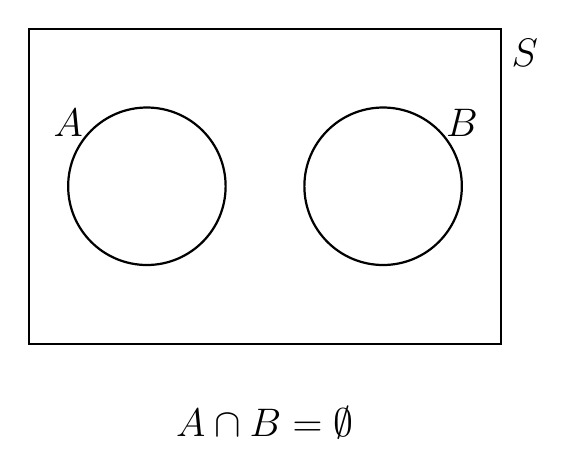
\begin{tikzpicture}
    % Draw sample space
    \draw[thick] (-1.5,-2) rectangle (4.5,2) node[below right] {\Large $S$};

    % Draw circles
    \draw[thick] (0,0) circle (1cm) node[left=1cm, above=0.5cm] {\Large $A$};
    \draw[thick] (3,0) circle (1cm) node[right=1cm, above=0.5cm] {\Large $B$};
  
    % Label mutually exclusive condition
    \node at (1.5, -3) {\Large $A \cap B = \emptyset$};
\end{tikzpicture}

\subsection*{Independent Events}

We usually use $P(A \mid B) = P(A)$ and  $P(B \mid A) = P(B)$ to check
if two events are independent.

\[P(A \cap B) = P(A) \cdot P(B)\]

\section*{Counting Principles}

Rule of Sum, Rule of Product, Permutations, Combinations

\subsection*{Rule of Product}

\subsection*{Permutations}

\[ P(n, r) = n \cdot (n-1) \cdot \dots \cdot (n-r+1) = \frac{n!}{(n-r)!} \]

\textbf{Theorem:} Number of permutations of $n$ distinct objects arranged in a \textbf{circle} is $(n-1)!$.

\subsection*{Combinations}

\[ C(n, r) = \frac{P(n, r)}{r!} = \frac{n!}{r!(n-r)!} \]

\section*{Finding Probability}

Generally, we need to list and find sample space, then count the number of favorable outcomes and find the probability.

If the experiment meets some attributes, we can use the following methods:

\subsection*{Binomial Distribution}

If the experiment meets the following conditions:

\begin{itemize}
    \item The experiment is repeated $n$ times.
    \item Each trial has two outcomes: success or failure.
    \item The probability of success is $p$ and the probability of failure is $q = 1 - p$.
    \item The trials are independent.
\end{itemize}

\subsection*{}

\end{document}